\documentclass[a4paper,10pt]{article}

\usepackage[utf8]{inputenc}
\usepackage[T1]{fontenc}
\usepackage{lmodern}
\usepackage{geometry}
\geometry{letterpaper}

\usepackage{doc}
\usepackage{url}

\usepackage{graphicx}
\usepackage{epstopdf}
\DeclareGraphicsRule{.tif}{png}{.png}{`convert #1 `dirname #1`/`basename #1 .tif`.png}


\geometry{hscale=0.85,vscale=0.85,centering}
\title{Protocole}
\author{Jean-Baptiste Dalle - Romain Gaborieau - Kevin Hivert - Alexis Braine}
\date{}

\begin{document}

\maketitle
\abstract{ Nous allons décrire dans la suite de ce document le protocole mis en place au sein de l'application de dessin collaboratif. Le protocole à été mis en place afin de permettre la connexion et la déconnexion d'un utilisateur, la transmission du dessin en temps réel entre tous les utilisateurs de l'application, la prise de contrôle sur le dessin en cours d'un utilisateur, etc... }


\section{Format des messages échangés.}
Afin de communiquer entre les clients et le serveurs nous avons définis un format précis de messages à envoyer qui permettra de savoir qui a envoyé le message d'une part et de faire passer une commande / une instructions et éventuellement (suivant le type de la commande) des paramètres ou des informations complémentaires. \\ \\


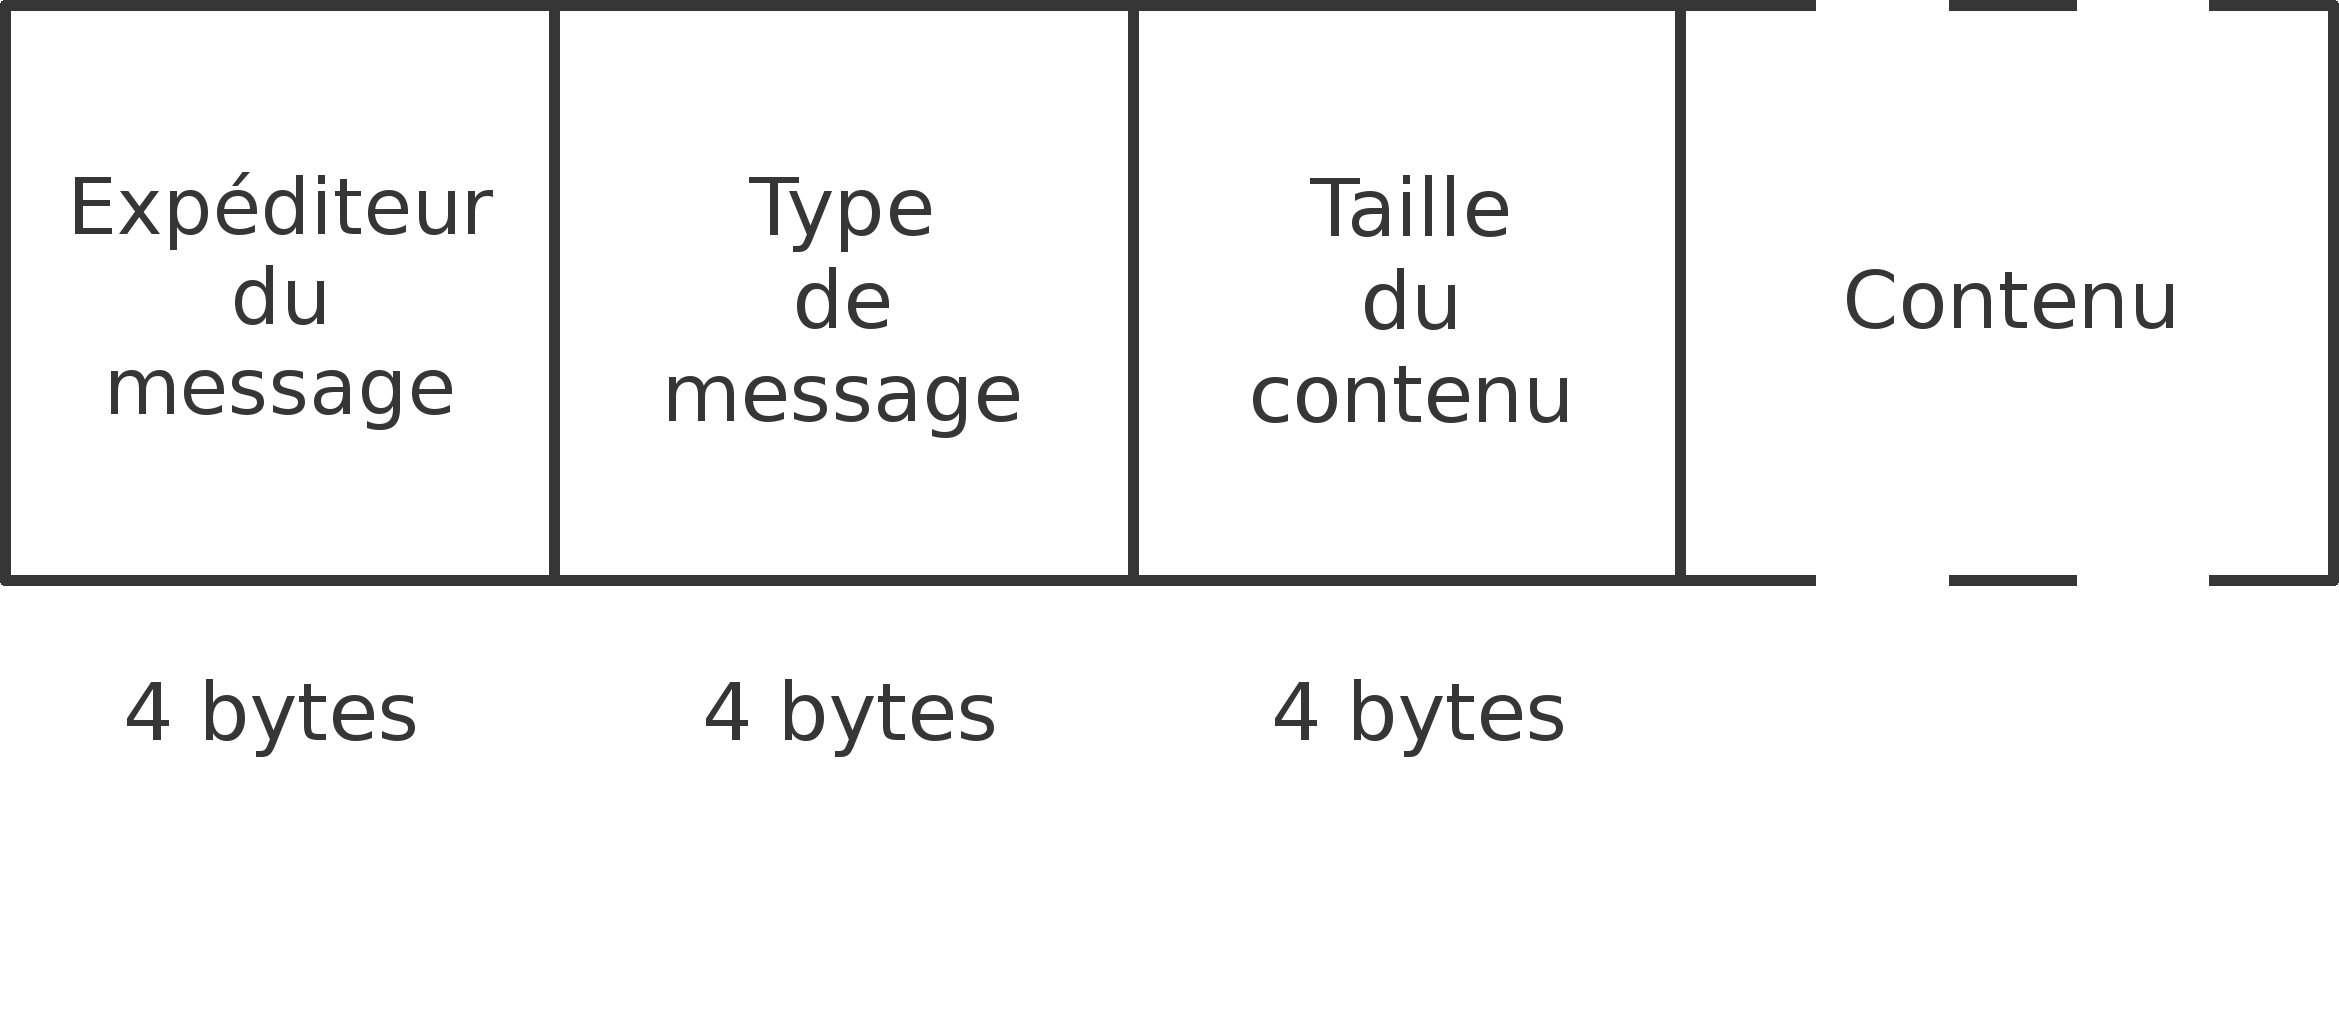
\includegraphics[scale=0.5]{message.png}

\paragraph{}Les messages sont donc constitués de quatre parties : 
\begin{itemize}
\item[1] L'adresse du destinataire, sur 4 octets.
\item[2] Le type de la commande, sur 4 octets également.
\item[3] La taille du contenu du message stocké sur 4 octets.
\item[4] Enfin, le contenu du message.
\end{itemize}


\paragraph{}\textit{Du point de programmation les messages sont stocké dans des byte[] et non pas de char[], car en Java un char est stocké sur 2 octets au lieu de 1. Pour des raisons de compatibilité avec d'autres langages nous avons donc pris la précaution de stocker les caractères des messages transmis sur des octets.}

\paragraph{}Le format ainsi construit des message nous permet donc aisément de savoir qui à envoyé le message et donc de lui répondre, d'envoyer des informations au client ou au serveur. Cela permet aussi au serveur d'envoyer des ordres aux clients (Le serveur peut indiquer à tout les clients que c'est au tour de tel client de prendre le contrôle du dessin), ainsi qu'au client d'envoyer des demandes au serveur (Le client peut demander à prendre la main par exemple).

\section{Types de messages échangés.}
\paragraph{}Afin de faire fonctionner notre application nous avons mis en place 13 commandes différentes qui vont être échangées entre les clients et la serveur.


\paragraph{}\begin{itemize}
\item CONNECT : Cette commande est utilisée par le client pour demander une connexion auprès du serveur. Cette commande est utilisée avec comme contenu de message le pseudo désiré par le client. Cette commande attend en retour, comme réponse soit la commande ACCEPT, soit la commande DENY que nous verons plus tard.

\item DISCONNECT : Cette commande est utilisée par le client pour se déconnecter. La commande n'attend rien en retour, le serveur en recevant le message retire le client de sa liste.

\item ACCEPT : Cette commande est envoyé par le serveur au client pour informer que le pseudo demander par le client et valide et que la connexion est accepté. Cette commande est aussi utilisé par le client pour informer le serveur qu'il est près à recevoir le dessin stocké sur le serveur.

\item DENY : Cette commande est envoyé par le serveur dans le cas où le pseudo demander par le client est déjà utilisé. Le client doit alors demander un autre pseudo.

\item  REQUEST$\_$CTRL : Il s'agit de la commande utilisé par les clients pour demander le contrôle du dessin.  Lorsqu'un client demande à prendre le contrôle du dessin le serveur l'ajoute à une liste d'attente, le client en tête de la liste obtient le contrôle pendant 30 secondes. A la fin du temps imparti, le client qui avait le contrôle est éliminé de la liste et on passe au client suivant, le client qui avait le contrôle doit donc redemander le contrôle pour être ré-inséré en fin de liste d'attente.

\item GIVE$\_$CTRL : Cette commande est utilisée par le serveur pour indiquer aux clients, qui prend le contrôle. 

\item LEAVE$\_$CTRL : Cette commande est envoyée du serveur au client qui a la main, afin qu'il la relâche,

\item SUBMIT : Cette commande est envoyé à chaque fois que le dessin est modifié. Le client qui a la main, l'envoie au serveur quand il fait une modification. Le contenu du message joint avec la commande est le contenu du dessin, c'est à dire le document SVG servant à le stocker.

\item UPDATE : Cette commande est renvoyé par le serveur à tous les client après qu'il ait reçu une modification du dessin de la part du client qui a le contrôle du dessin. Comme pour la commande SUBMIT, le contenu du message est le document SVG qui stocke le dessin.
On envoie également cette commande lorsque le client se connecte et qu'il a indiqué avec la commande ACCEPT, qu'il était près à recevoir le dessin.

\item GET$\_$USERS : Les clients utilisent cette commande pour demander la liste des utilisateurs connectés. Nous n'utilisons actuellement pas cette commande dans notre application, mais elle pourrait très bien servir pour afficher la liste complète des utilisateurs à chaque client et pourrait permettre d'ajouter un tchat à notre application de dessin.

\item LIST$\_$USERS : La commande devait servir de réponse à GET$\_$USERS, le contenu du message contient la liste des utilisateurs dans la même room que le client qui reçoit le message.

\item LIST$\_$ROOMS : Cette commande est envoyée par le serveur au client demandant une connexion afin qu'il puisse choisir une room dans la liste. Une room représentant un serveur avec un dessin différent stocké sur chaque room.
Nous n'avons cependant pas eu le temps d'implémenter complètement cette fonctionnalité à notre application, nous n'utilisons donc qu'une seule et unique room.

\item JOIN$\_$ROOM : Cette commande est utilisé par le client pour indiquer au serveur quelle room il veut rejoindre, et donc sur quel dessin il veut travailler.
\end{itemize}

\section{Déroulement du protocole}
\paragraph{}Nous allons maintenant suivre dans cette partie le déroulement du protocole depuis la connexion d'un client jusqu'à la modification du dessin et les répercutions de cette modification sur les autres clients.

\paragraph{}

\end{document}